\documentclass[conference,a4paper]{IEEEtran}
\IEEEoverridecommandlockouts

\usepackage{cite}
\usepackage{amsmath,amssymb}
\usepackage{graphicx}
\usepackage{array}
\usepackage{booktabs}
\usepackage[table]{xcolor}
\usepackage{url}
% allow long URLs in the references to break after any character
\makeatletter
\g@addto@macro{\UrlBreaks}{\do\-\do\_\do\a\do\b\do\c\do\d\do\e\do\f\do\g\do\h\do\i\do\j\do\k\do\l\do\m\do\n\do\o\do\p\do\q\do\r\do\s\do\t\do\u\do\v\do\w\do\x\do\y\do\z\do\0\do\1\do\2\do\3\do\4\do\5\do\6\do\7\do\8\do\9}
\makeatother
\usepackage{tikz}
\usetikzlibrary{positioning,fit,arrows.meta,calc}

% Two outputs from one source:
%   pdflatex saifa_telfor_v3.tex                                -> clean version
%   pdflatex -jobname=saifa_telfor_v3_izmene saifa_telfor_v3.tex -> changes marked
\newif\ifizmene
\edef\izmenejob{\detokenize{saifa_telfor_v3_izmene}}
\edef\currentjob{\jobname}
\ifx\izmenejob\currentjob \izmenetrue \fi
% \chg: changes made for the reviewers (blue)
% \dop: items filled in from documentation (green)
% \todo: still missing, must be resolved before submission (red, always shown)
\DeclareRobustCommand{\chg}[1]{\ifizmene{\color{blue}#1}\else#1\fi}
\DeclareRobustCommand{\dop}[1]{\ifizmene{\color{green!45!black}#1}\else#1\fi}
\DeclareRobustCommand{\todo}[1]{{\color{red}#1}}
% coverage marks for Table II
\newcommand{\cfull}{\tikz[baseline=-0.6ex]\fill (0,0) circle (2.1pt);}
\newcommand{\chalf}{\tikz[baseline=-0.6ex]{\draw[line width=0.4pt] (0,0) circle (2.1pt); \fill (0,0) -- (90:2.1pt) arc[start angle=90, end angle=270, radius=2.1pt] -- cycle;}}
\newcommand{\cnone}{\tikz[baseline=-0.6ex]\draw[line width=0.4pt] (0,0) circle (2.1pt);}

\begin{document}

\title{AI Gateways for EuroHPC AI Factories and Antennas: Functions, Tools and the SAIFA Example%
\thanks{This work has received funding from the European High Performance Computing Joint Undertaking (JU) under Grant Agreement No.~101263280 (SAIFA).}}

\author{
\IEEEauthorblockN{Aleksandra Stojanovi\'c}
\IEEEauthorblockA{\textit{School of Electrical Engineering} \\
\textit{University of Belgrade}\\
Belgrade, Serbia \\
sa230234d@student.etf.bg.ac.rs}
\and
\IEEEauthorblockN{Dimitrije Pe\v{s}i\'c}
\IEEEauthorblockA{\textit{School of Electrical Engineering} \\
\textit{University of Belgrade}\\
Belgrade, Serbia \\
pd230014d@student.etf.bg.ac.rs}
\and
\IEEEauthorblockN{Zaharije Radivojevi\'c}
\IEEEauthorblockA{\textit{School of Electrical Engineering} \\
\textit{University of Belgrade}\\
Belgrade, Serbia \\
zaki@etf.rs}
}


\maketitle
\bstctlcite{IEEEexample:BSTcontrol}

\begin{abstract}
The EuroHPC AI Factories initiative has built a network of AI supercomputing centres in Europe, and AI Factory Antennas bring their services to countries without large AI infrastructure. Users may therefore have to deal with several access points, \chg{from EuroHPC access calls and the EuroHPC Federation Platform to Factory contact offices, national Antennas and the AI-on-Demand Platform}. This paper gives an overview of these access points and proposes a general model of an \emph{AI gateway}, the part of an AI Factory or Antenna that users work with to reach computing, data, models, workflows, training and support. \chg{The main contribution is a clear division of responsibilities: what the gateway does itself, what it leaves to existing systems, and which system has the final word on access, resource allocation and accounting.} We define ten groups of functions, \chg{compare them with Waldur, Open OnDemand and the EuroHPC Federation Platform,} and list possible open-source tools. As an example, we use the gateway of the Serbian AI Factory Antenna (SAIFA), linked with Pharos and IT4LIA.
\end{abstract}

\begin{IEEEkeywords}
AI Factory, AI Factory Antenna, AI gateway, EuroHPC, federation, high-performance computing, MLOps, science gateway.
\end{IEEEkeywords}

\section{Introduction}

Modern artificial intelligence (AI) research needs large computing resources. To give such resources to more users, the EuroHPC Joint Undertaking (JU) started the AI Factories initiative. By October 2025, 19 AI Factories had been selected. Each of them has an AI supercomputer and offers data, model development, training and expert support~\cite{eurohpc_aif,eurohpc_six_aif}. In October 2025, 13 AI Factory Antennas were also selected to bring these services to more countries. Each Antenna is linked with one or more AI Factories~\cite{eurohpc_antennas,eurohpc_antennas_page}.

With so many sites, access becomes harder for users. Startups, small and medium-sized enterprises (SMEs), researchers and public institutions have to use several portals, accounts, application procedures and service lists before they can run one experiment. Science gateways solved a similar problem for grid and high-performance computing (HPC) resources by giving users simple web access~\cite{wilkinsdiehr2007,hudak2018ood}. AI Factories \chg{also} have to support the whole process of building a model, safe sharing of data and models, inference with large language models (LLMs), training for beginners, and work across national and European sites.

\chg{The main contribution of this paper is a general model of an AI gateway with a clear division of responsibilities: which functions the gateway performs itself, which it leaves to existing systems, and which system makes the final decision on access, resource allocation and accounting (Section~\ref{sec:model}). The model holds for an AI Factory and for an Antenna, whose main extra task is to connect its users with several Factories. We also compare its ten function groups with existing solutions. The gateway of the Serbian AI Factory Antenna (SAIFA)~\cite{cordis_saifa,saifa_d31} is used as an example.}

\section{How Users Access AI Factories Today}

\subsection{AI Factories}
AI Factories are run by national host organisations around EuroHPC supercomputers. The JU lists eight types of services they offer, \chg{from expert help and AI supercomputers to data management, training, middleware and AI software}~\cite{eurohpc_aif_services}. Computing time is given through EuroHPC access calls, \chg{in an} \emph{Industrial Innovation} mode with several sub-modes and a \emph{Science and Collaborative} mode~\cite{eurohpc_aif_access}. Each Factory also has its own contact office and its own rules for users. For example, the Greek Pharos Factory plans a Front Desk as the main point of contact~\cite{eurohpc_pharos}, and the Italian IT4LIA Factory offers its services for free to eligible users~\cite{eurohpc_it4lia}.

\subsection{AI Factory Antennas}
Antennas extend the services of existing AI Factories~\cite{eurohpc_antennas_page}. An Antenna usually offers a national entry point, smaller local computing resources, AI test environments, help for specific sectors and training. For large jobs it uses the linked Factories. One Factory can work with several Antennas \chg{and vice versa: Pharos} works with four Antennas (Pharos-CY, CALYPSO, VEZILKA and SAIFA), and the Swiss Antenna HEARTS \chg{with} four Factories~\cite{eurohpc_antennas}.

\subsection{Shared European platforms}
The first version of the EuroHPC Federation Platform (EFP) was \chg{released} in April 2026. It gives one entry point to several EuroHPC systems, with one login, common rules for resource allocation and data transfer, and a shared software catalogue. AI Factories will be added in later versions~\cite{eurohpc_efp}. The AI-on-Demand Platform is a European catalogue where users can find AI resources~\cite{aiod}. Table~\ref{tab:landscape} gives a short overview of all access points.

\begin{table}[!h]
\centering
\caption{Access points in the AI Factory network}
\label{tab:landscape}
\footnotesize
\renewcommand{\arraystretch}{1.1}
\begin{tabular}{@{}p{2.25cm}p{5.75cm}@{}}
\toprule
\textbf{Access point} & \textbf{What it offers to the user} \\
\midrule
EuroHPC access calls & Applying for computing time (industry and science modes) \\
EuroHPC Federation Platform & One login, common resource allocation and data transfer, shared software catalogue for EuroHPC systems \\
AI Factory contact office & Consulting, expert help, training, data services and computing at a national site \\
AI Factory Antenna & National entry point, local computing, help for new users, sending users and results to linked Factories \\
AI-on-Demand Platform & European catalogue of AI resources \\
\bottomrule
\end{tabular}
\end{table}

\chg{These access points cover different needs, but} none of them gives users one place where they can work with national resources, data, models and support and also reach the European services. This is the task of the AI gateway described in the next section.

\section{General Model of an AI Gateway}
\label{sec:model}

An AI gateway works as \emph{middleware} (Fig.~\ref{fig:arch}). It receives requests from users or applications, applies the same rules for identity, access and metadata to all of them, and sends each request to the right service. The gateway handles login and access control, the catalogue, checking and routing of requests, quotas, job status, monitoring, audit logs and data origin. It does not replace schedulers, storage systems, model servers, learning systems or partner platforms. Domain logic stays with the domain applications or with the users' own code.

\begin{figure}[t]
\centering
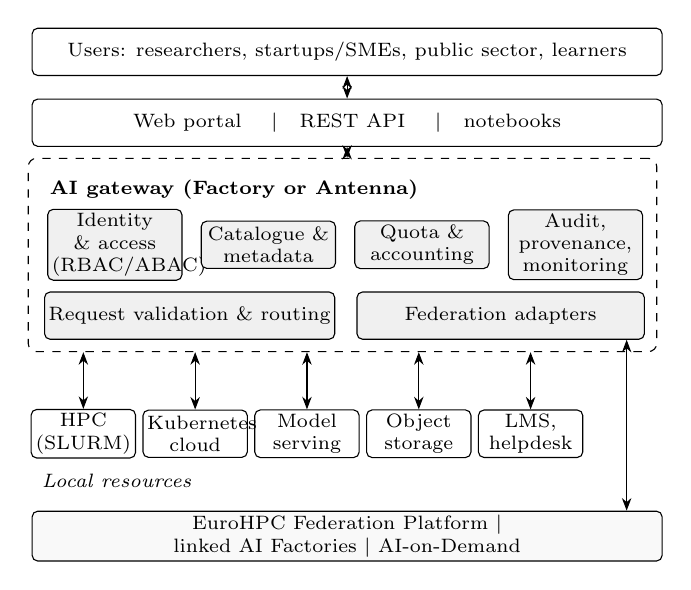
\begin{tikzpicture}[
  font=\scriptsize,
  box/.style={draw, rounded corners=2pt, align=center, minimum height=6mm, inner sep=1.5pt},
  core/.style={box, fill=gray!12},
  >={Stealth[length=1.6mm]}
]
\node[box, minimum width=8cm] (users) at (4,0) {Users: researchers, startups/SMEs, public sector, learners};
\node[box, minimum width=8cm] (portal) at (4,-0.9) {Web portal \quad\textbar\quad REST API \quad\textbar\quad notebooks};
\node[font=\scriptsize\bfseries, anchor=west] (gwt) at (0.1,-1.75) {AI gateway (Factory or Antenna)};
\node[core, text width=1.6cm] (iam)   at (1.05,-2.45) {Identity \& access\\(RBAC/ABAC)};
\node[core, text width=1.6cm] (cat)   at (3.0,-2.45) {Catalogue \&\\metadata};
\node[core, text width=1.6cm] (quota) at (4.95,-2.45) {Quota \&\\accounting};
\node[core, text width=1.6cm] (audit) at (6.9,-2.45) {Audit, provenance,\\monitoring};
\node[core, minimum width=3.65cm] (route) at (2.0,-3.35) {Request validation \& routing};
\node[core, minimum width=3.65cm] (fed)   at (5.95,-3.35) {Federation adapters};
\node[draw, dashed, rounded corners=3pt, fit=(gwt)(iam)(audit)(route)(fed), inner sep=1.5mm] (gw) {};
\foreach \n/\x/\t in {hpc/0.65/{HPC\\(SLURM)}, k8s/2.07/{Kubernetes\\cloud}, serve/3.49/{Model\\serving}, store/4.91/{Object\\storage}, lms/6.33/{LMS,\\helpdesk}}
  \node[box, minimum width=1.3cm, text width=1.22cm] (\n) at (\x,-4.85) {\t};
\node[font=\scriptsize\itshape, anchor=west] at (0,-5.45) {Local resources};
\node[box, minimum width=8cm, fill=gray!5, text width=7.8cm] (aif) at (4,-6.15) {EuroHPC Federation Platform \textbar\ linked AI Factories \textbar\ AI-on-Demand};
\draw[<->] (users) -- (portal);
\draw[<->] (portal) -- (portal |- gw.north);
\foreach \n in {hpc,k8s,serve,store,lms} \draw[<->] (gw.south -| \n) -- (\n);
\draw[<->] (7.55,-3.35 |- fed.south) -- (7.55,-3.35 |- aif.north);
\end{tikzpicture}
\caption{General model of an AI gateway between users, local resources and European AI Factory services.}
\label{fig:arch}
\end{figure}

The ten function groups in Table~\ref{tab:func} come from the SAIFA design (Section~\ref{sec:saifa}). Three rules apply to all groups: the server checks permissions for every action, every dataset, model and result has a version and a record of where it came from, and every job is checked against the user's quota before it starts.

\chg{Responsibilities follow the design baseline in~\cite{saifa_d31}. The institutional or EuroHPC identity provider authenticates the user, and the gateway links this identity to its own account.} \dop{The project owner invites members and assigns roles, and an organisation representative manages membership and allocations.} \chg{A partner AI Factory authorises the use of its resources, while the gateway only brokers the user's identity. Quota and accounting logic belongs to the gateway, which} \dop{keeps the record of available quota,} \chg{reserves allocation before a job is queued and records inference consumption. The gateway keeps metadata, review decisions, job records, audit and lineage, but takes job status from the scheduler} \dop{or the partner site}\chg{, which remains authoritative. The quota hierarchy, review states and responsibility matrix with operators are still being validated~\cite{saifa_d31}.}

\begin{table}[t]
\centering
\caption{Main function groups \chg{and their coverage by existing solutions}}
\label{tab:func}
\footnotesize
\renewcommand{\arraystretch}{1.0}
\setlength{\tabcolsep}{3pt}
\begin{tabular}{@{}>{\raggedright\arraybackslash}p{1.6cm}p{5.7cm}ccc@{}}
\toprule
\textbf{Group} & \textbf{Main features} & \chg{\textbf{W}} & \chg{\textbf{O}} & \chg{\textbf{E}} \\
\midrule
Identity \& access & Institutional (eduGAIN) and EuroHPC sign-in, account linking, RBAC/ABAC, scoped API tokens, revocation & \chg{\chalf} & \chg{\chalf} & \chg{\cfull} \\
Organisations \& projects & Workspaces, membership, roles, resource visibility (private, project, platform, public) & \chg{\cfull} & \chg{\cnone} & \chg{\chalf} \\
Catalogue & Search of models, datasets, workflows, services and courses; source attribution of federated entries & \chg{\chalf} & \chg{\cnone} & \chg{\chalf} \\
Data \& model management & Resumable upload, versioning, model and data cards, review and publication workflow & \chg{\cnone} & \chg{\chalf} & \chg{\chalf} \\
Compute jobs & Job templates, quota reservation, routing to HPC or Kubernetes, status, logs, result retrieval & \chg{\chalf} & \chg{\cfull} & \chg{\dop{\cfull}} \\
Inference & Authenticated, rate-limited access to served models and LLMs & \chg{\cnone} & \chg{\cnone} & \chg{\cnone} \\
Experiments \& MLOps & Experiment tracking, run comparison, benchmark evaluation, lineage across job, dataset and model & \chg{\cnone} & \chg{\cnone} & \chg{\cnone} \\
Training & Courses, learning paths, preconfigured notebook labs with controlled resources & \chg{\cnone} & \chg{\dop{\chalf}} & \chg{\cnone} \\
Operations & Monitoring, usage accounting, audit trail, notifications, contextual helpdesk tickets & \chg{\chalf} & \chg{\cnone} & \chg{\dop{\chalf}} \\
Federation & Catalogue exchange, metadata mapping, identity brokering, cross-factory execution and accounting & \chg{\chalf} & \chg{\dop{\cnone}} & \chg{\dop{\chalf}} \\
\bottomrule
\end{tabular}

\vspace{3pt}
\parbox{\columnwidth}{\scriptsize\raggedright \chg{W: Waldur, O: Open OnDemand}\dop{~\cite{hudak2018ood,chalker2018ood}}\chg{, E: EFP}\dop{~\cite{eurohpc_efp_page}}\chg{. \cfull{} provided, \chalf{} partly (configuration or extension), \cnone{} not provided (new development).}}
\end{table}

\begin{table*}[t]
\centering
\caption{Possible tools for each part and work needed for the gateway}
\label{tab:tools}
\footnotesize
\renewcommand{\arraystretch}{1.0}
\setlength{\tabcolsep}{4pt}
\newcommand{\grp}[1]{\multicolumn{3}{|l|}{\cellcolor{gray!12}\textbf{\textit{#1}}} \\ \hline}
\begin{tabular}{|>{\raggedright\arraybackslash}p{2.9cm}|>{\raggedright\arraybackslash}p{7.0cm}|>{\raggedright\arraybackslash}p{6.5cm}|}
\hline
\rowcolor{gray!30}
\textbf{Part} & \textbf{Main option (alternatives)} & \textbf{Work needed for the gateway} \\ \hline
\grp{User access}
Portal \& UX & Next.js/React (Nuxt/Vue) & Unified UI, backend-for-frontend, tool embedding \\ \hline
Identity \& policies & Keycloak (authentik, WSO2 IS); Open Policy Agent (Casbin, Cedar) & Role mapping, ABAC attributes, account linking, policy model \\ \hline
Notebooks & JupyterHub + KubeSpawner (SlurmSpawner, code-server) & Launch from portal, quotas, dataset mount, audit \\ \hline
\grp{Data and models}
Catalogue \& search & CKAN or Dataverse (DataHub, OpenMetadata); OpenSearch + pgvector & Unified catalogue, ACL filtering in index, federation \\ \hline
Model registry \& experiments & MLflow (ClearML, Aim) & Model cards, approval workflow, access rights \\ \hline
Storage & PostgreSQL, S3-compatible object store (MinIO/Ceph), Valkey & Metadata links, lifecycle, retention \\ \hline
Lineage & OpenLineage + Marquez & Links between jobs, datasets, models and results \\ \hline
\grp{Compute and inference}
LLM inference \& serving & vLLM (TGI, SGLang, Triton); KServe (Ray Serve, BentoML) & API proxy, quotas, routing, audit \\ \hline
Fine-tuning & Hugging Face TRL/PEFT (Axolotl, LLaMA-Factory) & Approved templates, HPC submission, result registration \\ \hline
HPC \& batch & SLURM, Open OnDemand; Kubernetes Jobs (Volcano, Kueue) & HPC bridge, unified job model, SLURM/K8s routing \\ \hline
Workflows \& containers & Argo Workflows (Airflow, Flyte); Harbor + Trivy, Apptainer on HPC & Workflow templates, image approval and HPC conversion \\ \hline
\grp{Operations and federation}
Observability \& audit & Prometheus, Grafana, Loki, OpenTelemetry; append-only log + WORM archive & Correlation with user/job, shared audit events \\ \hline
Learning \& support & Moodle (Open edX); Zammad or GLPI & Portal links, lab quotas, contextual tickets \\ \hline
Federation \& accounting & DCAT/DCAT-AP adapters (CKAN harvester); Waldur as cross-layer option & Partner adapters, per-factory accounting \\ \hline
\end{tabular}
\end{table*}

\section{Description of the Main Functions}

\subsection{Login, access and collaboration}
Users log in with their university or institute account (for example through eduGAIN) or with a EuroHPC account, and the gateway connects these logins to one user account. Access is decided by the user's role and by other attributes, such as organisation, project and type of data~\cite{nist_abac}. Seeing a resource in the catalogue and using it are two separate permissions, \chg{and search never shows resources of other projects that the user may not use.}

\subsection{Datasets and models}
\chg{Formal review is tied to publication~\cite{saifa_d31}. Training needs only access to a dataset, runs can be repeated freely, and artefacts are linked automatically to the dataset, configuration and job. A dataset or model version is published only after a data administrator or model reviewer approves it, and the decision is recorded. Only published resources can be exported to partners.} Large files are uploaded in parts with checksums \chg{and stored as immutable versions}. Published resources have FAIR metadata~\cite{wilkinson2016fair}, which also makes it easier to share them with partner catalogues.

\subsection{Jobs, inference and experiments}
Before a job starts, the gateway checks the input data and the user's access, and reserves quota. Then it sends the job to HPC through SLURM~\cite{yoo2003slurm} or to Kubernetes~\cite{burns2016borg}. Sensitive data can stay where it is, and the job is sent to the data. The scheduler still manages the queue. The gateway collects status, logs and results and shows them in the same way for all systems, and containers are converted to Apptainer/Singularity images~\cite{kurtzer2017singularity} for HPC. Requests to a model go through a proxy that checks the user and the limits and charges the quota before the request is sent on. A person always decides which model to keep.

\subsection{Working with partners: Factory and Antenna}
A Factory mostly \emph{publishes} its services and resources to European platforms. An Antenna also has to \emph{connect} its users with one or more linked Factories. It converts user identities and metadata, sends large test jobs to a partner site, returns the results to the user's project, and keeps track of usage for each Factory. Each partner is connected through its own catalogue adapter, for example using DCAT~\cite{w3c_dcat3}. Resources from partners keep their source and are never changed locally. The first connections are read-only or simulated, so the gateway keeps working when a partner is down. When AI Factories are added to the EFP~\cite{eurohpc_efp}, gateways should use its login and allocation services instead of building their own.

\section{\chg{Existing Solutions and} Possible Tools}

\chg{Three existing solutions already cover part of the model: Waldur, a platform for projects, allocation and accounting on cloud and HPC systems~\cite{waldur_docs}; Open OnDemand, a web portal for HPC centres~\cite{hudak2018ood}; and the EFP~\cite{eurohpc_efp}, itself built on MyAccessID, Waldur and Open OnDemand~\cite{nortamo2025efp}; Table~\ref{tab:func} shows their coverage. Login, projects, allocation, accounting and interactive HPC work mostly need configuration. None of them covers the AI-specific functions (dataset and model review, inference with quotas, experiment lineage) or sends an Antenna's work to linked Factories with usage kept for each Factory. These functions, and the shared rules for access, quotas and metadata, are what the model adds and where most new development is needed.}

\chg{Existing tools are used first, and new ones are built only when needed.} Table~\ref{tab:tools} gives the main option for each part, alternatives in brackets, and the work that each gateway still has to do itself. Most options are well known open-source projects, for example JupyterHub~\cite{kluyver2016jupyter,jupyterhub_docs}, MLflow~\cite{zaharia2018mlflow}, vLLM~\cite{kwon2023vllm} and Open OnDemand~\cite{hudak2018ood}.

Tools are chosen in two steps. First, each tool must meet the basic requirements for its area, \chg{for example login through both SAML2 and OIDC linked to one account, immediate revocation of access, and one adapter for each new partner.} Second, the tools that pass are compared by ease of use, \chg{integration and operating effort,} speed and cost, maturity, and legal issues (GDPR, data location, licences). Open-source tools that can run on our own servers are preferred.

\section{Example: SAIFA}
\label{sec:saifa}

SAIFA, \chg{the Serbian Antenna linked with Pharos and IT4LIA, runs} from May 2026 to April 2029~\cite{cordis_saifa}. Its local resources are the PARADOX HPC cluster at the Institute of Physics Belgrade and the AI infrastructure of the Institute for AI Research and Development of Serbia. The function groups in Table~\ref{tab:func} were made from 23 user stories in \chg{its four domains (language and culture, energy and manufacturing, health, environment),} such as flood prediction with AutoML, synthetic genome sequencing data, hate-speech detection in Serbian and simulation of social networks with LLM agents, \chg{and then turned} into 20 system use cases~\cite{saifa_d31}.

The SAIFA design proposes a basic proof-of-concept setup to test the candidate tools together: a web portal, login through home institutions, an access-control module, PostgreSQL with S3 storage, JupyterHub, a model-serving service, a separate bridge to SLURM, and Prometheus/Grafana monitoring. For each part, it must show where data is stored, how identity is passed on, how resources are charged and logged, how access is checked and what happens when another service fails~\cite{saifa_d31}. The beta version of the gateway is planned for April 2027 and must offer at least one full path for a user: log in, find a resource, run a job and follow its progress.

\section{Conclusion}

\chg{The main contribution of this paper is a model of an AI gateway with a clear division of responsibilities between the gateway, existing systems and partner Factories. The comparison with Waldur, Open OnDemand and the EFP shows that mainly the AI-specific functions and the work with several Factories need new development. Open questions are how gateways will use the EFP for login and allocation, how to track usage across several Factories, which common metadata to use for models and datasets, and which data rules apply when jobs run in another country. Next, we will report on the SAIFA beta version and on tests with Pharos and IT4LIA.}

\bibliographystyle{IEEEtran}
\bibliography{references_v3}

\end{document}
